\documentclass{article}


\usepackage[utf8]{inputenc}
\usepackage[T1]{fontenc}
\usepackage[a4paper,includeheadfoot,margin=2.54cm,includehead]{geometry}
\usepackage[skip=2mm, indent=5mm]{parskip}
\usepackage[sfdefault]{notomath}
\usepackage{float}
\usepackage{graphicx}
\usepackage[figurename=Fig.]{caption}
\usepackage[unicode,bookmarks,colorlinks,breaklinks]{hyperref}  
\usepackage{color}
\usepackage{fancyhdr}


\begin{document}

% ------------------------------------------------
% | % Título, autor, materia, fecha, ciudad... % |
% ------------------------------------------------
\newcommand{\titulo}{Documentación del proyecto Boxing Game}
\newcommand{\escuela}{Escuela de Ingeniería Informática}
\newcommand{\autorAngel}{Ángel Iglesias Préstamo}
\newcommand{\autorDiego}{Diego Martín Fernández}
\newcommand{\asignatura}{Informática Audiovisual}
\newcommand{\universidad}{Universidad de Oviedo}
\newcommand{\fecha}{\today} % Muestra por defecto la fecha actual

% ----------------------------------------------------------
% | % Establecemos un estilo para el encabezado y el pie % |
% ----------------------------------------------------------
\pagestyle{fancy}
\fancyhf{}

\renewcommand{\headrulewidth}{0.5pt}
\renewcommand{\footrulewidth}{0.5pt}

\fancyhead[RO]{\nouppercase{\titulo\hfill\asignatura}}
\fancyfoot[CE,CO]{\thepage}

% --------------------------------------------------------------------
% | % Establecemos el estilo de los enlaces y referencias-cruzadas % |
% --------------------------------------------------------------------

\definecolor{blueUniovi}{RGB}{0,51,170}
\hypersetup{
    linkcolor=blueUniovi,
    citecolor=blueUniovi,
    filecolor=black,
    urlcolor=blueUniovi,
    bookmarksnumbered=true,
    bookmarksopen=true,
    bookmarksopenlevel=1,
    pdfpagemode=UseOutlines
}

% --------------------------------------------------------------
% | % Establecemos el estilo de algunas secciones y párrafos % |
% --------------------------------------------------------------

\makeatletter
\renewcommand\paragraph{\@startsection{paragraph}{4}{\z@}%
    {3.25ex \@plus1ex \@minus.2ex}%
    {0pt}%
    {\normalfont\normalsize\bfseries}}
\makeatother

% -----------------------------
% | % Portada del documento % |
% -----------------------------
\newcommand{\HRule}{\rule{\linewidth}{0.5mm}}
\begin{titlepage}
    \centering
    
\includegraphics[width=0.3\textwidth]{img/uniovi}
    \vfill
    \HRule
    \vspace{0.4cm}
    {\huge\bfseries\titulo\par}
    \vspace{1.5cm}
    {\Large\itshape\autorAngel\par\vspace{0.1cm}\autorDiego\par}
    \vspace{0.4cm}
    \HRule
    \vspace{1.5cm}
    {\LARGE\escuela\par}
    \vspace{0.5cm}
    {\Large\asignatura\par}
    \vfill
    {\large\universidad\par}
    \fecha
    \vfill
\end{titlepage}

% -----------------------------------------
% | % Tabla de contenidos del documento % |
% -----------------------------------------
\thispagestyle{empty}
\renewcommand{\contentsname}{Tabla de contenidos}
\tableofcontents{}
\newpage
\setcounter{page}{1}

% ---------------------------------------
% | % Empezamos el documento en sí :D % |
% ---------------------------------------

\section{Introducción}

\href{https://angelip2303.github.io/boxing-docs/}{Boxing Game} es el proyecto en equipo de la asignatura de Informática Audiovisual desarrollado por Ángel Iglesias Préstamo y Diego Martín Fernández. Se trata de un mini-juego de boxeo controlado mediante una cámara. La presente es la documentación del mismo. En esta se desarrolla el proceso seguido para diseñar el sistema en el apartado \ref{section:design}. En la sección \ref{section:development} se describe el proceso seguido para la correcta implementación del mini-juego planteado en el punto anterior: esto es, un breve comentario acerca de las tecnologías utilizadas. Posteriormente, en el apartado \ref{section:manual} se redactan una serie de consideraciones a tener en cuenta para poder interactuar correctamente con el sistema. Finalmente, en la sección \ref{section:work}, se justifica el trabajo aportado por cada uno de los miembros del equipo.

\section{Diseño}
\label{section:design}

\subsection{Diagramas}

\subsubsection{Diagrama de clases}

\begin{figure}[H]
    \centering
    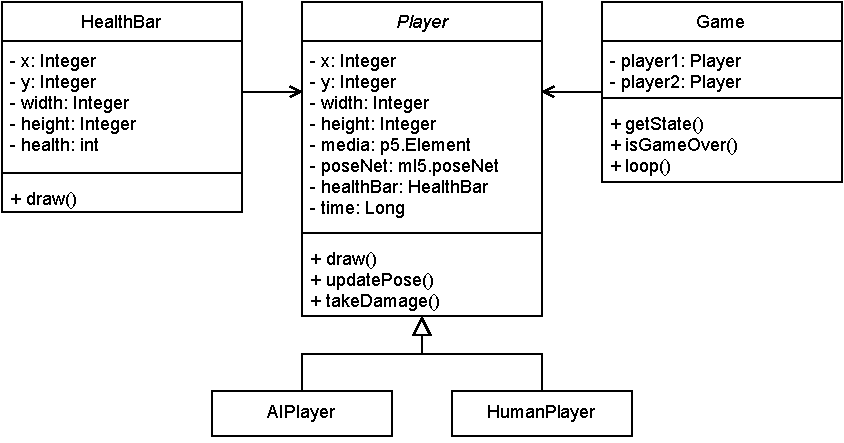
\includegraphics[width=\textwidth]{img/class-diagram}
    \caption{Diagrama de clases del sistema que hemos desarrollado}
    \label{fig:class-diagram}
\end{figure}

El diagrama \ref{fig:class-diagram} se muestra la clase \texttt{Game} que se encarga de la lógica del juego y los eventos desde la función \texttt{loop()}, tales como si el juego está acabado o no. Por otra parte, tenemos una clase \texttt{Player} de la que extendemos las distintas implementaciones como \texttt{AIPlayer} y \texttt{HumanPlayer}. Además, estas se encargan de la lógica relativa a detección de posición. Más sobre esto en la sección \ref{section:ml5}. Por último, la clase \texttt{HealthBar} forma parte de las anteriormente mencionadas, y se encarga de dibujar la vida en la pantalla y llevar el conteo de la misma: interfaz de usuario.

\subsubsection{Wireframe}

En el diagrama \ref{fig:wireframe} se presenta un pequeño diseño de la pantalla principal del juego -- donde -- se muestra la disposición que seguiremos cuando implementemos el sistema. Al ser tan sencillo, realmente no es fundamental crear esta guía; sin embargo, hay varias consideraciones que merece la pena destacar. La primera, hemos decidido colocar al jugador que juega en local; esto es, el jugador humano, a la izquierda de la pantalla: ya que en occidente se lee de izquierda a derecha, y está pensado para ser jugado por personas relativas a la asignatura. Además, y como mencionaremos más adelante, destaca el uso del rojo como color para acentuar peligro y la barra de vida. También, es importante destacar que estas se encuentran en la parte superior de la pantalla porque hemos utilizado referencias traídas de otros juegos de combate: \textit{Street Fighter}, y por convenio y familiaridad de los posibles jugadores, creemos que es la mejor idea.

\begin{figure}[H]
    \centering
    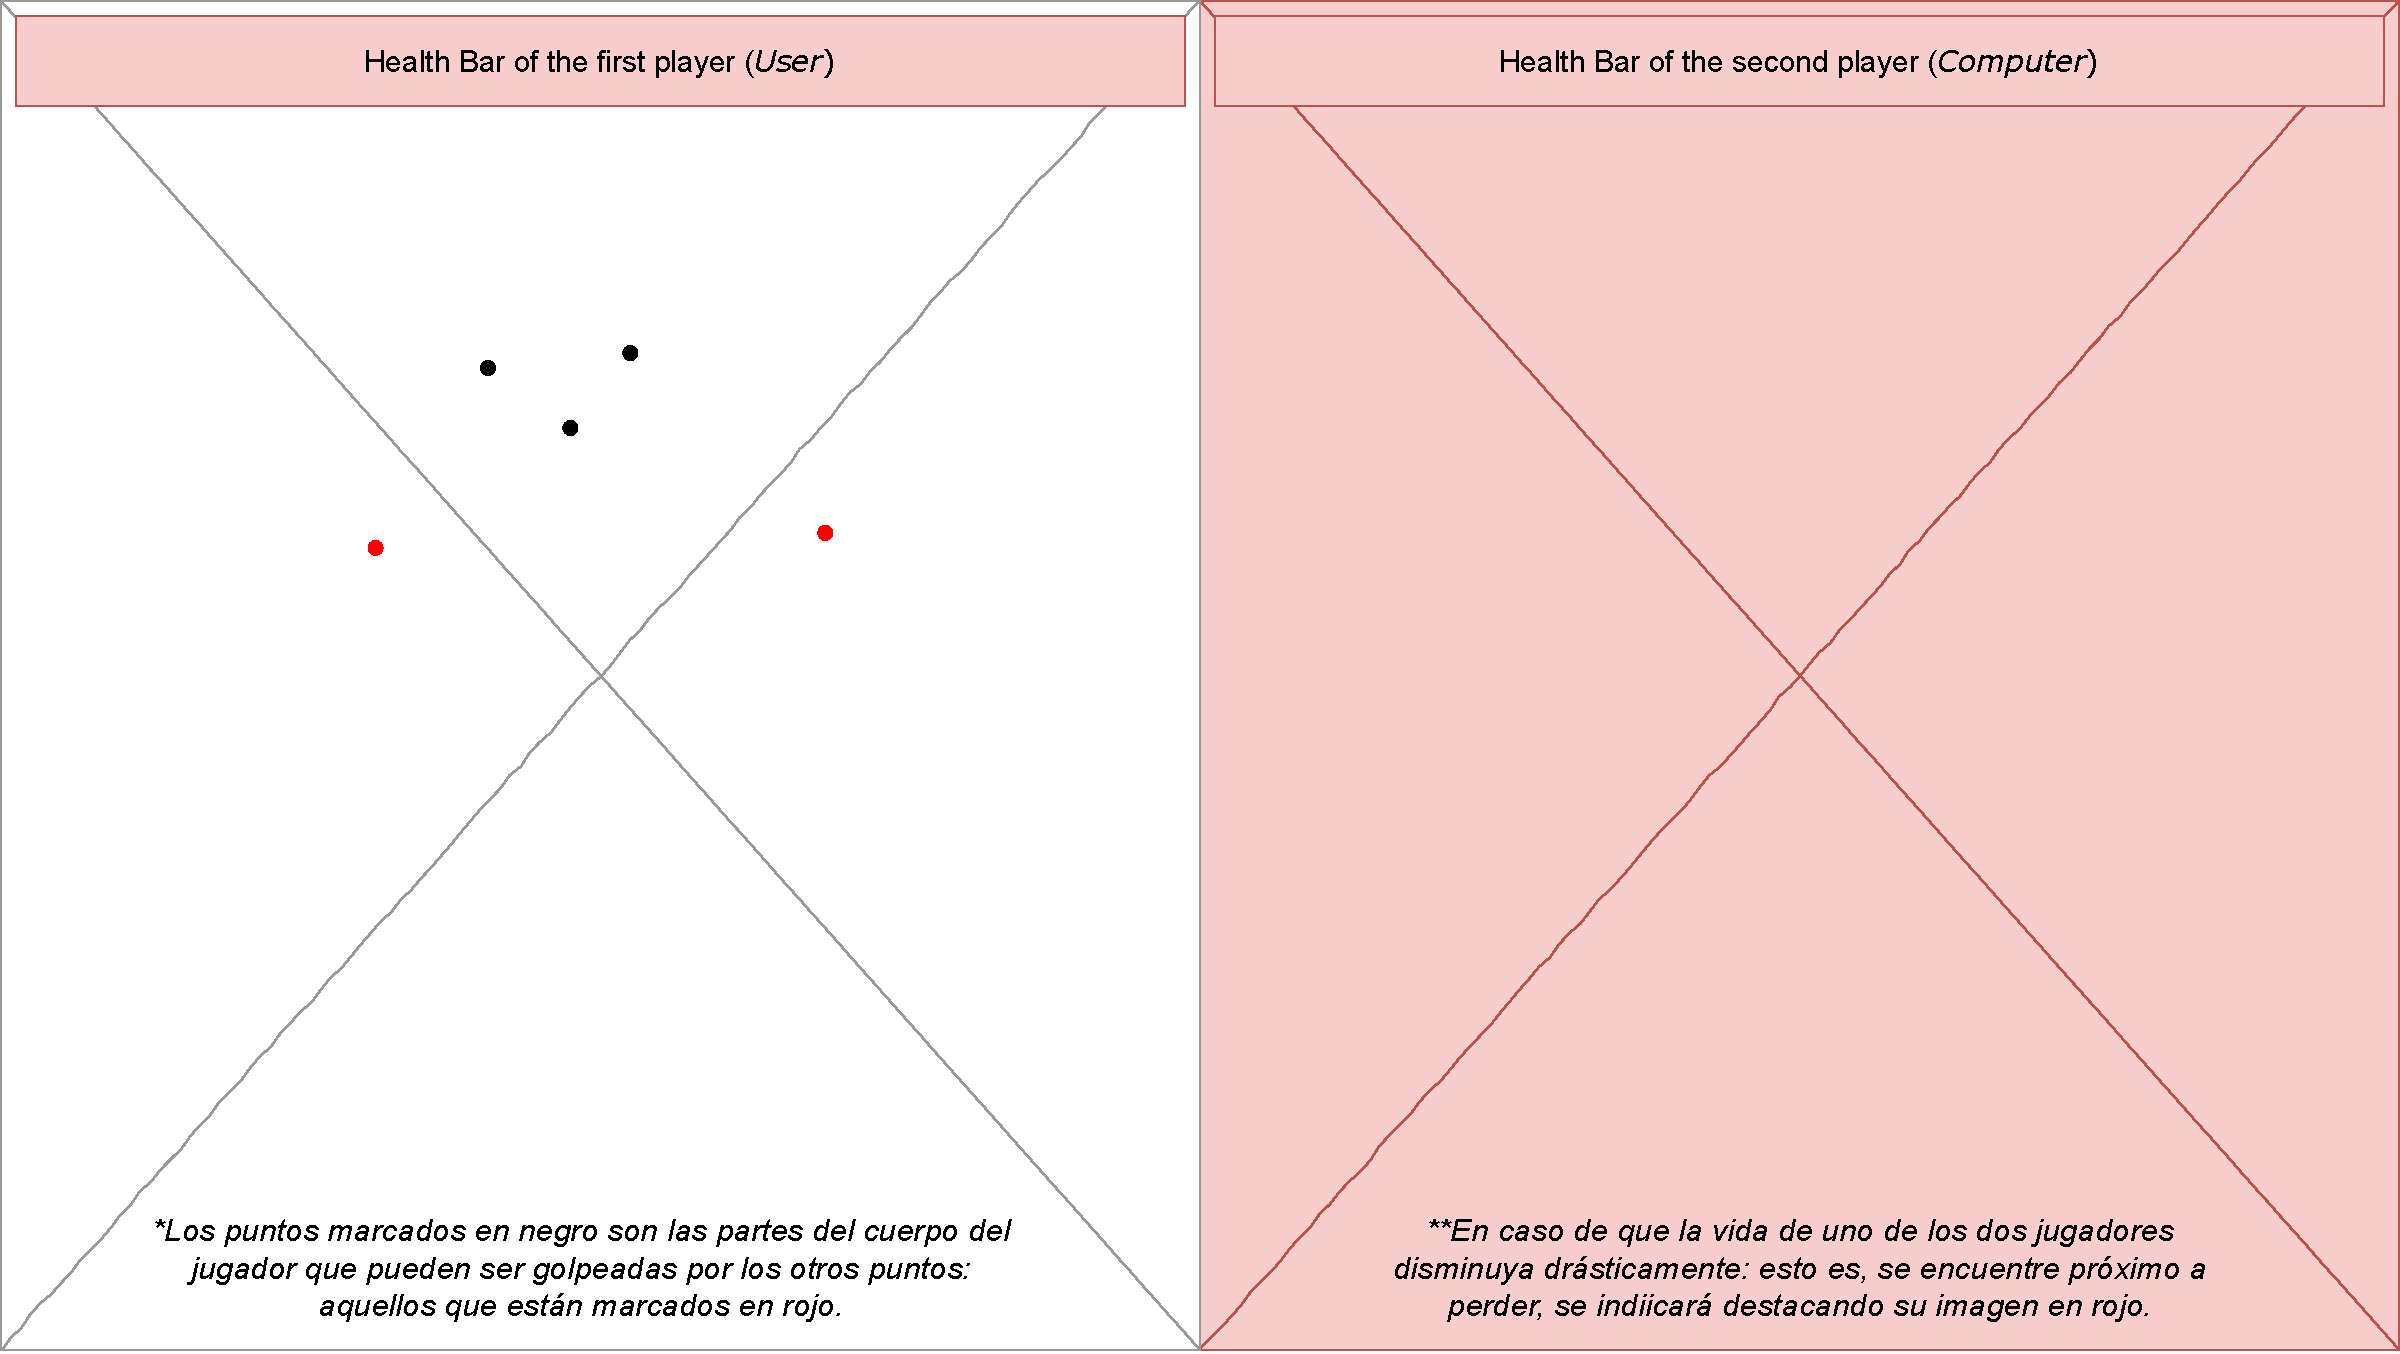
\includegraphics[width=\textwidth]{img/wireframe}
    \caption{Wireframe de la pantalla principal de la interfaz de usuario}
    \label{fig:wireframe}
\end{figure}

\subsection{Colores}

Hemos decidido utilizar un rojo para destacar que un determinado jugador corre peligro: esto es, que está cerca de perder. Para ser más concretos, el rojo que hemos empleado es \texttt{RGB(255, 0, 0)} con cierta opacidad para permitir ver lo que hay detrás. De esta forma, utilizamos este color como símbolo de violencia o sangre. Más allá de este, hemos coloreado las partes que pueden ejercer un daño en rojo, mientras que las que pueden ser dañadas en blanco. De acuerdo con la simbología, el primero hace referencia a la violencia, mientras que el segundo lo hace a la paz, esto es, partes del cuerpo que no dañan. En la pantalla final se muestran letras blancas sobre un fondo negro -- para maximizar el contraste -- además de que este último es símbolo de muerte: final de partida. En esta documentación y en las diapositivas se usa el azul como único color para acentuar los enlaces, ya que por convenio es el que se suele utilizar: familiaridad.

Resumiendo todo, puede ser un sistema sencillo, pero un concienzudo análisis previo sobre colores, formas y simbología puede ayudar a la hora de permitir a los jugadores usarlo sin necesidad de recurrir a guías o manuales. Así pues, el objetivo es que pueda ser lo más usable posible.

\subsection{Tipografía}

La tipografías utilizadas son sans-serif para facilitar la legibilidad en dispositivos electrónicos. Con esto le damos un toque informal al proyecto debido a la temática del mismo, un videojuego. Además, usamos una fuente \texttt{monospace} para destacar elementos propios del mundo de la Informática informática como código, entre otros. Además usamos \textit{cursiva} para anglicismos y tecnicismos de otra índole.

\section{Desarrollo}
\label{section:development}

\subsection{Tecnologías utilizadas}

\subsubsection{p5.js}

\href{https://p5js.org/es/}{p5.js} es la biblioteca de JavaScript que hemos utilizado en la asignatura para desarrollar proyectos de programación creativa. En nuestro caso, nos ha permitido implementar un sistema audiovisual donde el usuario interactúa mediante una cámara conectada a su dispositivo. Podríamos resumir el uso que le damos a \textit{p5.js} como el marco de trabajo para permitir la interacción cliente-sistema y viceversa. No sólo se puede controlar al jugador, sino que también se recibe información sobre el estado de la partida: una barra de vida, colores que nos destacan las partes del cuerpo que golpean y las que pueden ser golpeadas; más de eso en la sección \ref{section:design}.

\subsubsection{ml5.js}
\label{section:ml5}

\href{https://ml5js.org/}{ml5.js} es una biblioteca de JavaScript que permite el desarrollo de aplicaciones que exploren el uso de inteligencia artificial en el navegador. La mayor ventaja, en nuestro caso, que presenta es que permite una integración muy sencilla con \textit{p5.js}. De esta forma, permite el uso del modelo \texttt{ImageNet} para la detección de \textit{Poses}: esto es, nos facilita la detección de las partes del cuerpo de sendos jugadores.

De alguna forma podríamos decir que el \textit{stack} formado por las dos tecnologías mencionadas es realmente el núcleo del proyecto.

\section{Futuras ampliaciones}

Hemos coincidido que en el futuro no estaría mal realizar las siguientes ampliaciones que, por falta de tiempo, no ha sido imposible realizar.

\begin{itemize}
    \item \textbf{PvP (Pelea entre dos humanos)}: se podría usar una sola cámara que grabara a dos personas. Estando en el mismo lugar pero en seciones separadas de la pantalla. Un ejemplo sería que la parte izquierda de la grabación hiciera el reconocimiento de una persona y la parte de la derecha a la otra.
    \item \textbf{Hacer que la IA también golpee}: ahora mismo la única forma de recibir daño es que nos agachemos y choquemos contra los puños de la IA, pero esta podría devolver los golpes. Se podría hacer un modelo 3D estilo boxeo de la Wii.
    \item \textbf{Juego en línea contra otra persona}.
    \item \textbf{Ranking}: hacerlo de forma competitiva con divisiones, de esta forma estaríamos alargando la vida del juego y crearíamos una comunidad.
    \item \textbf{Mejorar el sistema de daño}: de esta forma, golpear distintas partes del cuerpo infringiría una cantidad de daño distinta, en vez de que todos los golpes sean iguales.
\end{itemize}

\section{Manual}
\label{section:manual}

\subsection{Requisitos}

\paragraph{Activar la aceleración por Hardware} \mbox{} -- Para alcanzar el mayor rendimiento de la aplicación se recomienda activar la aceleración por Hardware. Esto permite al sistema el uso de la GPU para que esta se encargue de ejecutar el modelo de aprendizaje automático \texttt{ImageNet} para la detección de \textit{Poses}. Se deben seguir los siguientes pasos:

\begin{enumerate}
    \item Acceda a la configuración de su navegador.
    \item Busque \textit{Aceleración por Hardware} y active esa funcionalidad.
\end{enumerate}

\paragraph{Permitir el uso de la cámara} \mbox{} -- La forma en la que se interactúa con el sistema es a través de la cámara. Es por eso que se deberá permitir el uso de la misma para poder jugar a \textit{Boxing Game}.

\subsection{Uso}
El modelo clasifica las partes del cuerpo del jugador, por lo que lo único que tenemos que hacer es mover los puños de forma que hagan daño al rival. Este recibe daño cuando uno de nuestros puños -- representados por puntos rojos en la pantalla -- hace colisión con el cuerpo del rival: representados por los puntos blancos. Estas colisiones tienen un margen de error -- en torno a un radio -- para que sea más fácil acertar un impacto. El jugador que primero se quede sin vida es el perdedor.

\section{Reparto del trabajo}
\label{section:work}
Inicialmente, Ángel creó los repositorios y se encargó de realizar un \textit{modelo mínimo viable} que luego fue ampliado por Diego: depurándolo y mejorándolo en general. Además, Ángel se encargó del despligue y la integración continua del sistema. Diego grabó y editó el vídeo promocional. Finalmente, la presentación se hizo conjuntamente. Si bien la documentación fue realizada por Ángel.

\end{document}
